\documentclass[11pt,fleqn]{article}

\setlength {\topmargin} {-.15in}
\setlength {\textheight} {8.6in}

\usepackage{amsmath}
\usepackage{amssymb}
\usepackage{color}
\usepackage{tikz}
\usetikzlibrary{automata,positioning,arrows}
\usepackage{diagbox}



\newcommand{\be}{\begin{enumerate}}
\newcommand{\ee}{\end{enumerate}}

\begin{document}
\begin{center}
	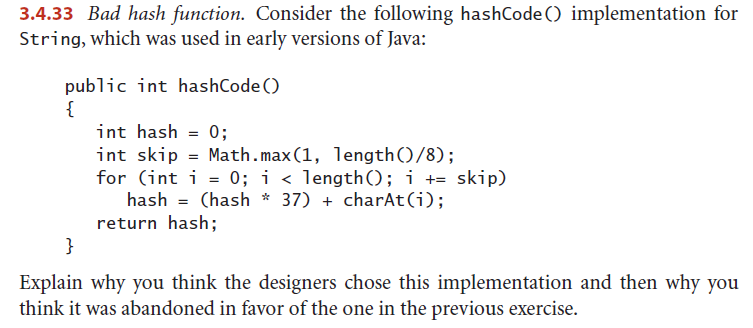
\includegraphics[scale=.85]{3.4.33.png}
\end{center}
	
\textbf{Solution:}\\
\begin{itemize}
	\item This method skips some characters, so distribution of values trying to hash may not be correct.
	\item Computation time will be faster because less characters to check.
	\item This is used for longer strings with some identical elements at same place. So it's not good to hvae because missing some characters since 'skips' at length 8.
\end{itemize}

\begin{center}
	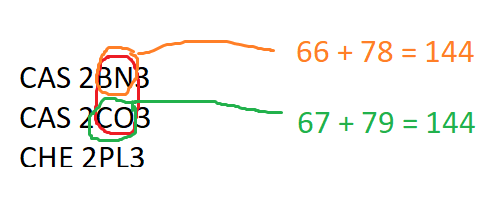
\includegraphics[scale=.85]{3.4.33-SOLN.png}
\end{center}
	


\end{document}
